\section{OD requirements}

\par
As previously stated, the primary purpose of the OD is to act as an active veto for neutrons.
Practically, this means that there are a number of performance requirements which the OD has to meet, all of which can be found in \cite{LZ_TechnicalDesignReview_ref}.
A subset, which are address in this Thesis are presented in Table \ref{tab:veto_requirements}.

\begin{table}[!htbp]
    \centering
    \begin{tabular}{p{0.3\textwidth}p{0.6\textwidth}} %{ c | c {\textwidth} } 
    \hline
    {Requirement Number} & {Description} \\ \hline
    R-160001             & Detection efficiency of 95\% for a 1 MeV neutron that scatters once in the xenon \\
    R-160005             & Must not veto more than 5\% of the WIMP search live-time
    \end{tabular}
    \caption{Selection of the OD veto performance requirements. Adapted from Table 12.2.6 from \cite{LZ_TechnicalDesignReview_ref}}
    \label{tab:veto_requirements}
\end{table} 

\par
The veto method adopted for SR1 is to act as a 'dumb' veto, as no attempt will be made to determine that cause of light seen in the OD.
This means that an event will be vetoed if the following two conditions are met;

\begin{enumerate}
    \item A pulse is seen with an energy above the veto threshold.
    \item The pulse is within the veto window.
\end{enumerate}

The two requirements in Table \ref{tab:veto_requirements} are clearly intertwined.
The veto window and threshold are primarily determined by the background rate in the OD in order to reduce the impact on live-time.
This does however need to be balanced to maintain a suitable veto efficiency.

\subsection{OD Backgrounds}
\par
A background in the OD is any event that is not what it was designed to detect and veto - so any event that is not a neutron or $\gamma$ that has scattered once in the TPC.
There sources of backgrounds are; Cavern-$\gamma$'s, impurities in the GdLS and other detector components.
The rate of backgrounds in the OD is expected to be largely made up from two sources; cavern-$\gamma$'s and internal contaminants. 

\subsubsection{Cavern-$\gamma$'s}
\par
Due to the results of the LS Screener campaign, a dedicated Cavern-$\gamma$ study was undertaken as mentioned in Section \ref{sec:cavern_gamma_generator}.
This showed that the rate of these $\gamma$'s may in fact be $\approx$50\% of what was anticipated in the TDR.
However, this remains a significant uncertainty.
They are expected to be the dominant effect at higher energies (>2MeV)




\subsubsection{GdLS impurities}
\par
In order to ascertain the rate of internal contaminants expected, a campaign was undertaken \cite{scotthaselschwardt_thesis_ref} to determine this expected rate.
The results from this are shown in table \ref{tab:gdls_assay_rates}.
\par
One of the key outcomes of the screener campaign were the high ${}^{235}U$ rate.
As such, the method of doping the LS was altered, which aimed to reduce the contamination.
The expected rates from this are also shown in Table \ref{tab:gdls_assay_rates}.
However, as these were not screened the accuracy is unknown, but gives a 'best-case'.


\begin{table}[!htbp]
    \centering
    \begin{tabular}{c|c|c}
        \multirow{2}{*}{Isotope or Subchain}  &  \multicolumn{2}{c}{GdLS rates (mBq/kg)}      \\ 
                             &  LS Screener          & Improved Purification \\ \hline
        ${}^{238}U_{e}$      &  $< 1.04$             & $< 0.017$             \\ 
        ${}^{238}U_{m}$      &  $0.092\pm0.02$       & $0.010\pm0.004$       \\
        ${}^{235}U_{e}$      &  $0.011$              & $< 0.018$             \\
        ${}^{235}U_{l}$      &  $0.10\pm0.04$        & $< 0.012$             \\
        ${}^{232}Th_{e}$     &  $< 0.027$            & $< 0.0036$            \\
        ${}^{232}Th_{l}$     &  $< 0.020$            & $< 0.0030$            \\
        ${}^{40}K$           &  $< 0.22$             & $< 0.0092$            \\
        ${}^{138}La$         &  $< 0.0055$           & $< 0.0017$            \\
        ${}^{176}Lu$         &  $0.30\pm0.07$        & $0.0081\pm0.0018$     \\
        ${}^{152}{Gd}$       &  $1.61\pm0.08$        & $1.61\pm0.08$         \\
        ${}^{152}{Sm}$       &  $1.02\pm0.05$        & $1.02\pm0.05$         \\
        ${}^{14}{C14}$       &  $4.77\pm0.098$       & $4.77\pm0.098$ 
    \end{tabular}
    \caption{Activities of GdLS components during LS Screener testing and those projected from an improved purification technique. Values from Table 4.9 and 6.11 of \cite{scotthaselschwardt_thesis_ref}}
    \label{tab:gdls_assay_rates}
\end{table}


\subsubsection{LZ Detector Components}
\par
A third source are decays originating from other components which are all contaminated with ${}^{238}U$ and ${}^{232}Th$ at a minimum from exposure to the cavern.
The most significant other decay of note is ${}^{60}Co$ from the OCV with an expected activity of XXX \cite{LZ_assay_ref}.


\subsubsection{Summary}
\par
A new set of simulations were performed to attain the expected rate of backgrounds.
These estimates are provided in Table \ref{tab:od_expected_rates}.
The lower rates from Table \ref{tab:gdls_assay_rates} are used to be more representative of what to expect from data.
The rates of LZ components and Cavern-$\gamma$'s differ here compared to previous background studies such as in \cite{LZ_TechnicalDesignReview_ref,LZ_projected_sensitivity_paper_ref,scotthaselschwardt_thesis_ref} as the simulated OD geometry has improved and more sources have been taken into account.

\begin{table}[!htbp]
    \centering
    \begin{tabular}{c|c|c|c|c} %{ c | c {\textwidth} } 
    \hline
    \multirow{2}{*}{Source} & \multicolumn{4}{c}{Rate (Hz)} \\
                            & All   & $>$ 100 keV & $>$ 200 keV & $>$ 2 MeV \\ \hline
    Cavern-$\gamma$         & 80.7  & 55.5        & 44.7        & 4.6       \\
    LZ components           & 29.6  & 25.4        & 21.0        & 0.9       \\
    GdLS Internals          & 40.2  & 24.5        & 11.9        & 0.0       \\
    Total                   & 148.2 & 90.3        & 62.7        & 13.2
    \end{tabular}
    \caption{Expected rate in the OD. !!TODO add uncertainty!!}
    \label{tab:od_expected_rates}
\end{table} 

\subsection{Efficiency}
\par
Neutron sources that can enter the TPC can originate from a ($\alpha$,n) reactions.
These are the most dangerous in terms of number expected, but also as only a single neutron will be released.
The primary other expected neutrons originate from spontaneous fission.
However multiple neutrons are released, often with higher energies and they are accompanied by $\gamma$'s and $\beta$'s so vetoing these is of less concern.

\begin{figure}[!htbp]
    \centering
    \begin{tikzpicture}
        \begin{axis}[
            xlabel=Energy (MeV),
            ylabel=Emission (arbitary units),
            width=15cm,
            height=6cm,
            xmin=0,
            xmax=10,
            ymin=0,]
            \addplot[red, const plot]
                    table [x=Energy,y=Rate]
                    {Data/Neutrons/background_neutron_spectrum.dat};
        \end{axis}
    \end{tikzpicture}
    \caption{Expected distribution of neutron energies from ($\alpha$,n) and USF neutrons.}
    \label{fig:simulation_background_neutron_energies}
\end{figure}


\begin{equation}
    \epsilon = \frac{\text{events passing}\mathbf{SS, ROI, FID, Vetos}}{\text{events passing}\mathbf{SS, ROI, FID}}
    \label{eq:neutron_efficiency}
\end{equation}

\par
The neutron efficiency had been calculated in \cite{sallyshaw_thesis_ref}, however that was before construction has begun and so may not reflect the current status.
It as therefore redone in a similar fashion.
the OD geometry has changed significantly since then it has been re-done and additional detector efficiencies have been taken into account.
Previously, energy deposit simulations for background neutrons were used. 
From this, single scatters were isolated by XXX.
The skin cuts were defined as; XXX


\par
The same method has been applied here, however, the neutron source was changed to be 'post'-single scatter. 
As the neutron will not lose a significant amount of it's energy upon the scatter, a 1 MeV neutron will typically remain above XXX MeV...
Additionally, studying the efficiency in this regard allows for the requirement to be directly probed as well as studying how the neutron energy affects the efficiency.

\par
Figure \ref{fig:neutron_eff_energy_dep_tpc_neutrons} contains the result of this study alongside the previous result.
Firstly, it is important to note that the requirement R-160001 remains satisfied.
Secondly, the energy of the neutron is an important factor in the performance of the veto.
The expected energy spectrum for neutrons is shown in Figure \ref{fig:simulation_background_neutron_energies}.


\begin{tcolorbox}[colback=red!5!white, colframe=red!50!black, title=Key Plots]
\begin{enumerate}
    \item Simulation Efficiency
    \item Neutron capture energy deposits
    \item alpha,n energies
    \item fraction of gammas that get captured in the OD after SS (AmLi sims)
    \item fraction of neutrons that get captured in each volume
    \item time spent in volume vs OD capture time (for all and for Gd-only) to show what causes each component
    \item Energy deposited in OD vs veto time
\end{enumerate}
\end{tcolorbox}


\begin{figure}[!htbp]%
\centering
\begin{tikzpicture}
\centering
  \begin{groupplot}[%view={0}{90},
    group style = {group size = 2 by 2,vertical sep=1.5cm}]
    \nextgroupplot[
            title=TDR background neutrons,
            ylabel=Efficiency (\%),
            width=0.5\textwidth, height=6cm,
            xmin=0, xmax=1000,
            ymin=85, ymax=100,
            minor y tick num=4,
            grid=major]
            \addplot+[green, mark=none]
                    table [x=Time,y=Efficiency]
                    {Data/Neutron_Efficiency/Simulation/od_efficiency_sally_0kev.dat};
            \addplot[green, only marks,  mark size=1pt,
                     error bar legend,
                     error bars/.cd,
                     x dir=both, x explicit, error bar style={color=black}]
                    table [x=Time,y=Efficiency, x error=XError]
                    {Data/Neutron_Efficiency/Simulation/od_efficiency_sally_0kev.dat};
                    
            \addplot+[blue, mark=none]
                    table [x=Time,y=Efficiency]
                    {Data/Neutron_Efficiency/Simulation/od_efficiency_sally_100kev.dat};
            \addplot[blue, only marks,  mark size=1pt,
                     error bar legend,
                     error bars/.cd,
                     x dir=both, x explicit, error bar style={color=black}]
                    table [x=Time,y=Efficiency, x error=XError]
                    {Data/Neutron_Efficiency/Simulation/od_efficiency_sally_100kev.dat};
                    
            \addplot+[red, mark=none]
                    table [x=Time,y=Efficiency]
                    {Data/Neutron_Efficiency/Simulation/od_efficiency_sally_200kev.dat};
            \addplot[red, only marks,  mark size=1pt,
                     error bar legend,
                     error bars/.cd,
                     x dir=both, x explicit, error bar style={color=black}]
                    table [x=Time,y=Efficiency, x error=XError]
                    {Data/Neutron_Efficiency/Simulation/od_efficiency_sally_200kev.dat};
                    
    \nextgroupplot[
            title=100 keV,
            width=0.5\textwidth, height=6cm,
            xmin=0, xmax=1000,
            ymin=85, ymax=100,
            %yticklabels=\empty,
            yticklabel pos=right,
            minor y tick num=4,
            grid=major]
            \addplot+[green, smooth, mark=none]
                    table [x=Time,y=Efficiency]
                    {Data/Neutron_Efficiency/Simulation/edep_tpc_neutron_eff_100kev_threshold_0kev_smooth_line.dat};
            \addplot[green, only marks, mark size=1pt,
                     error bar legend,
                     error bars/.cd,
                     x dir=both, x explicit, error bar style={color=black}]
                    table [x=Time,y=Efficiency, x error=EfficiencyError]
                    {Data/Neutron_Efficiency/Simulation/edep_tpc_neutron_eff_100kev_threshold_0kev_error_bars.dat};
                    
            \addplot+[blue, smooth, mark=none]
                    table [x=Time,y=Efficiency]
                    {Data/Neutron_Efficiency/Simulation/edep_tpc_neutron_eff_100kev_threshold_100kev_smooth_line.dat};
            \addplot[blue, only marks, mark size=1pt,
                     error bar legend,
                     error bars/.cd,
                     x dir=both, x explicit, error bar style={color=black}]
                    table [x=Time,y=Efficiency, x error=EfficiencyError]
                    {Data/Neutron_Efficiency/Simulation/edep_tpc_neutron_eff_100kev_threshold_100kev_error_bars.dat};
                    
            \addplot+[red, smooth, mark=none]
                    table [x=Time,y=Efficiency]
                    {Data/Neutron_Efficiency/Simulation/edep_tpc_neutron_eff_100kev_threshold_200kev_smooth_line.dat};
            \addplot[red, only marks, mark size=1pt,
                     error bar legend,
                     error bars/.cd,
                     x dir=both, x explicit, error bar style={color=black}]
                    table [x=Time,y=Efficiency, x error=EfficiencyError]
                    {Data/Neutron_Efficiency/Simulation/edep_tpc_neutron_eff_100kev_threshold_200kev_error_bars.dat};

    \nextgroupplot[
            title=1 MeV,
            xlabel=Veto Window ($\mu$s),
            ylabel=Efficiency (\%),
            width=0.5\textwidth, height=6cm,
            xmin=0, xmax=1000,
            ymin=85, ymax=100,
            minor y tick num=4,
            grid=major,
            legend style = { column sep = 10pt, legend columns = -1, legend to name = Simulated_Neutron_Eff_CommonLegend,}]
            \addplot+[green, smooth, mark=none]
                    table [x=Time,y=Efficiency]
                    {Data/Neutron_Efficiency/Simulation/edep_tpc_neutron_eff_1mev_threshold_0kev_smooth_line.dat};
            \addplot[green, only marks, mark size=1pt,
                     error bar legend,
                     error bars/.cd,
                     x dir=both, x explicit, error bar style={color=black}]
                    table [x=Time,y=Efficiency, x error=EfficiencyError]
                    {Data/Neutron_Efficiency/Simulation/edep_tpc_neutron_eff_1mev_threshold_0kev_error_bars.dat};
                    
            \addplot+[blue, smooth, mark=none]
                    table [x=Time,y=Efficiency]
                    {Data/Neutron_Efficiency/Simulation/edep_tpc_neutron_eff_1mev_threshold_100kev_smooth_line.dat};
            \addplot[blue, only marks,  mark size=1pt,
                     error bar legend,
                     error bars/.cd,
                     x dir=both, x explicit, error bar style={color=black}]
                    table [x=Time,y=Efficiency, x error=EfficiencyError]
                    {Data/Neutron_Efficiency/Simulation/edep_tpc_neutron_eff_1mev_threshold_100kev_error_bars.dat};
                    
            \addplot+[red, smooth, mark=none]
                    table [x=Time,y=Efficiency]
                    {Data/Neutron_Efficiency/Simulation/edep_tpc_neutron_eff_1mev_threshold_200kev_smooth_line.dat};
            \addplot[red, only marks, mark size=1pt,
                     error bar legend,
                     error bars/.cd,
                     x dir=both, x explicit, error bar style={color=black}]
                    table [x=Time,y=Efficiency, x error=EfficiencyError]
                    {Data/Neutron_Efficiency/Simulation/edep_tpc_neutron_eff_1mev_threshold_200kev_error_bars.dat};
            \legend{,0keV,,100keV,,200keV}                
    \nextgroupplot[
            title=6 MeV,
            xlabel=Veto Window ($\mu$s),
            width=0.5\textwidth, height=6cm,
            xmin=0, xmax=1000,
            ymin=85, ymax=100,
            %yticklabels=\empty,
            yticklabel pos=right,
            minor y tick num=4,
            grid=major,]
            \addplot+[green, smooth, mark=none]
                    table [x=Time,y=Efficiency]
                    {Data/Neutron_Efficiency/Simulation/edep_tpc_neutron_eff_6mev_threshold_0kev_smooth_line.dat};
            \addplot[green, only marks, mark size=1pt,
                     error bar legend,
                     error bars/.cd,
                     x dir=both, x explicit, error bar style={color=black}]
                    table [x=Time,y=Efficiency, x error=EfficiencyError]
                    {Data/Neutron_Efficiency/Simulation/edep_tpc_neutron_eff_6mev_threshold_0kev_error_bars.dat};
                    
            \addplot+[blue, smooth, mark=none]
                    table [x=Time,y=Efficiency]
                    {Data/Neutron_Efficiency/Simulation/edep_tpc_neutron_eff_6mev_threshold_100kev_smooth_line.dat};
            \addplot[blue, only marks, mark size=1pt,
                     error bar legend,
                     error bars/.cd,
                     x dir=both, x explicit, error bar style={color=black}]
                    table [x=Time,y=Efficiency, x error=EfficiencyError]
                    {Data/Neutron_Efficiency/Simulation/edep_tpc_neutron_eff_6mev_threshold_100kev_error_bars.dat};
                    
            \addplot+[red, smooth, mark=none]
                    table [x=Time,y=Efficiency]
                    {Data/Neutron_Efficiency/Simulation/edep_tpc_neutron_eff_6mev_threshold_200kev_smooth_line.dat};
            \addplot[red, only marks, mark size=1pt,
                     error bar legend,
                     error bars/.cd,
                     x dir=both, x explicit, error bar style={color=black}]
                    table [x=Time,y=Efficiency, x error=EfficiencyError]
                    {Data/Neutron_Efficiency/Simulation/edep_tpc_neutron_eff_6mev_threshold_200kev_error_bars.dat};
            \node[] at (axis cs: 600,90) {6 MeV};
  \end{groupplot}
   \node at ($(group c2r1) - (group c1r1) + (-0.5cm, 6.0cm)$) {\ref{Simulated_Neutron_Eff_CommonLegend}};
\end{tikzpicture}
\caption{Neutron Veto Efficiency using energy deposits. TDR-era result with incomplete and simpler geometry taken from \cite{sallyshaw_thesis_ref}.}
\label{fig:neutron_eff_energy_dep_tpc_neutrons}
\end{figure}

\par
Those this shows that there is good neutron efficiency, it does not tell the full story.
In fact only XXX \% of the neutrons get captured in the GdLS (from the 1MeV neutrons that start in the fiducial volume), and even if a neutron is captured, the released $\gamma$'s do not have to scatter within the GdLS.
The energy deposits that are observed come from $\gamma$'s released as a result of captures elsewhere.



\par
Something about where neutrons spend there time...

\subsection{Simulated Calibration Efficiency}
\par
Although the efficiency shown in energy deposit simulations shows that the requirement will be met, it will need to be confirmed during the calibration phase.
Therefore it is important to perform the same analysis with a simulated calibration source, and any differences be understood.

\par
The source chosen for this was AmLi.
AmLi is an ($\alpha$,n) source, producing neutrons predominantly under 0.5MeV with the full spectrum is shown in Figure \ref{fig:amli_neutron_energy_spectrum}.
This source was chosen over other neutron calibration sources (such as DD and ${}^{252}Cf$ as it will be used to tune the TPC interaction finding algorithms.
It also has the lowest computationally intensive of the available sources, allow for higher statistics in the simulations.

\begin{figure}[!htbp]
    \centering
    \begin{tikzpicture}
        \begin{axis}[
            xlabel=Energy (MeV),
            ylabel=Probability,
            width=15cm,
            height=6cm,
            xmin=0,
            ymin=0,]
            \addplot[red, const plot]
                    table [x=Energy,y=Probability]
                    {Data/Neutrons/amli_neutron_spectrum.dat};
        \end{axis}
    \end{tikzpicture}
    \caption{AmLi neutron energy. Data from \cite{amli_neutron_energy_ref} }
    \label{fig:amli_neutron_energy_spectrum}
\end{figure}

\par
Three source locations were chosen, all in CSD-1;
\begin{enumerate}
    \item \textbf{0mm:} In line with the cathode
    \item \textbf{700mm:} In the centre of the TPC
    \item \textbf{1400mm:} At the top of the TPC
\end{enumerate}
A graphical depiction is shown in Figure \ref{fig:CSD1_Geometry}. 

\begin{figure}[!htbp]
\centering
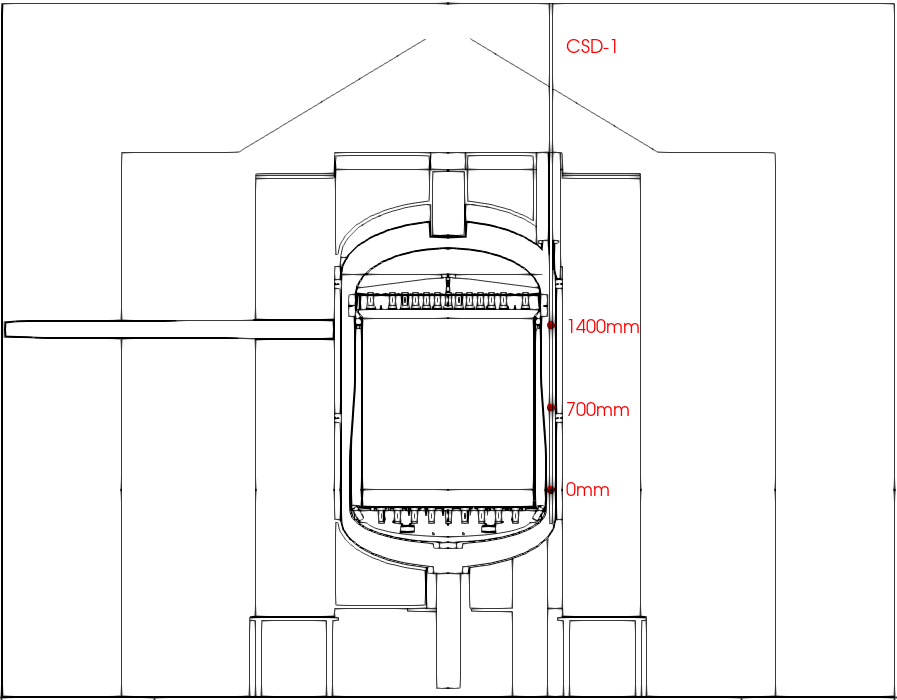
\includegraphics[width=\textwidth]{Figures/Geometry/csd1_geometry_black_and_white.png}
\caption{LZ geometry slice as implemented in GEANT4 from the water tank in. CSD-1 is shown along with the relevant Z-positions for calibration runs.}
\label{fig:CSD1_Geometry}
\end{figure}


\par
The result of the simulations are shown in Figure XXX and summarised in Table \ref{tab:amli_neutron_simulations_veto_efficiency}.

\begin{table}[!htbp]
    \centering
    \begin{tabular}{c|c|c|c|c|c|c}
         \multirow{2}{*}{Neutron Source} & \multicolumn{5}{c|}{Number passing cut}      & \multirow{2}{*}{Veto Eff. (\%)}  \\ 
                         & Simulated  & Usable     & SS        & FID     & Veto         &                                  \\ \hline
        energy dep       & 19,310,000 & 19,280,766 & 1,474,033 & 325,080 & 323,319      & 99.4                             \\
        full propagation & X          & X          &           &         &              & 
    \end{tabular}
    \caption{Number of events passing various cuts from AmLi simulation in CSD1.}
    \label{tab:amli_neutron_simulations_veto_efficiency}
\end{table}








\begin{figure}[!htbp]%
\centering
\begin{tikzpicture}
\centering
    \begin{groupplot}[%view={0}{90},
    group style = {group size = 2 by 2,vertical sep=1.5cm}]
    \nextgroupplot[
            xlabel=Veto Window ($\mu$s),
            ylabel=Efficiency (\%),
            width=0.5\textwidth, height=6cm,
            xmin=0, xmax=1000,
            ymin=85, ymax=100,
            minor y tick num=4,
            grid=major,
            legend style = { column sep = 10pt, legend columns = -1, legend to name = Simulated_AmLi_CommonLegend,}]
            \addplot+[green, mark=none]
                    table [x=Time,y=Efficiency]
                    {Data/Neutron_Efficiency/Simulation/edep_amli_neutron_eff_amli_edeps_threshold_0kev_error_bars.dat};
            \addplot[green, only marks, mark size=1pt,
                     error bar legend,
                     error bars/.cd,
                     x dir=both, x explicit, error bar style={color=black}]
                    table [x=Time,y=Efficiency, x error=EfficiencyError]
                    {Data/Neutron_Efficiency/Simulation/edep_amli_neutron_eff_amli_edeps_threshold_0kev_error_bars.dat};
                    
            \addplot+[blue, mark=none]
                    table [x=Time,y=Efficiency]
                    {Data/Neutron_Efficiency/Simulation/edep_amli_neutron_eff_amli_edeps_threshold_100kev_error_bars.dat};
            \addplot[blue, only marks, mark size=1pt,
                     error bar legend,
                     error bars/.cd,
                     x dir=both, x explicit, error bar style={color=black}]
                    table [x=Time,y=Efficiency, x error=EfficiencyError]
                    {Data/Neutron_Efficiency/Simulation/edep_amli_neutron_eff_amli_edeps_threshold_100kev_error_bars.dat};
                    
            \addplot+[red, mark=none]
                    table [x=Time,y=Efficiency]
                    {Data/Neutron_Efficiency/Simulation/edep_amli_neutron_eff_amli_edeps_threshold_200kev_error_bars.dat};
            \addplot[red, only marks, mark size=1pt,
                     error bar legend,
                     error bars/.cd,
                     x dir=both, x explicit, error bar style={color=black}]
                    table [x=Time,y=Efficiency, x error=EfficiencyError]
                    {Data/Neutron_Efficiency/Simulation/edep_amli_neutron_eff_amli_edeps_threshold_200kev_error_bars.dat};
            \legend{,0keV,,100keV,,200keV}
        \nextgroupplot[
            xlabel=Veto Window ($\mu$s),
            width=0.5\textwidth, height=6cm,
            xmin=0, xmax=1000,
            ymin=85, ymax=100,
            yticklabel pos=right,
            minor y tick num=4,
            grid=major]
            \addplot+[green, mark=none]
                    table [x=Time,y=Efficiency]
                    {Data/Neutron_Efficiency/Simulation/amli_neutron_eff_0kev_error_bars.dat};
            \addplot[green, only marks, mark size=1pt,
                     error bar legend,
                     error bars/.cd,
                     x dir=both, x explicit, error bar style={color=black}]
                    table [x=Time,y=Efficiency, x error=EfficiencyError]
                    {Data/Neutron_Efficiency/Simulation/amli_neutron_eff_0kev_error_bars.dat};
            \addplot+[blue, mark=none]
                    table [x=Time,y=Efficiency]
                    {Data/Neutron_Efficiency/Simulation/amli_neutron_eff_50kev_error_bars.dat};
            \addplot[blue, only marks, mark size=1pt,
                     error bar legend,
                     error bars/.cd,
                     x dir=both, x explicit, error bar style={color=black}]
                    table [x=Time,y=Efficiency, x error=EfficiencyError]
                    {Data/Neutron_Efficiency/Simulation/amli_neutron_eff_50kev_error_bars.dat};
            \addplot+[red, mark=none]
                    table [x=Time,y=Efficiency]
                    {Data/Neutron_Efficiency/Simulation/amli_neutron_eff_100kev_error_bars.dat};
            \addplot[red, only marks, mark size=1pt,
                     error bar legend,
                     error bars/.cd,
                     x dir=both, x explicit, error bar style={color=black}]
                    table [x=Time,y=Efficiency, x error=EfficiencyError]
                    {Data/Neutron_Efficiency/Simulation/amli_neutron_eff_100kev_error_bars.dat};
    \end{groupplot}
     \node at ($(group c2r1) - (group c1r1) + (-0.5cm, 5.0cm)$) {\ref{Simulated_AmLi_CommonLegend}};
\end{tikzpicture}
    \caption{Simulated AmLi neutron tagging efficiency. \textbf{Left:} energy deposits \textbf{Right:} Complete propagation and event reconstruction}
    \label{fig:simulated_amli_neutron_efficiency.}
\end{figure}

\par
Highlighting the difference in
Additionally, during the calibration data taking it will not be possible to have such ideal circumstances to test the neutron tagging performance.
Therefore, in order to quantify this, two neutron sources were simulated, AmLi and DD, the deployment methods of each are described in Section XXX.


Particularly given the propagation effects raised in Section XXX.
\par
In Chapter \ref{chap:analysis_of_the_od}, the requirements are tested in data.